\subsection{Sistema de Control}

Ahora, se deben diseñar los circuitos auxiliares del sistema de control que rodean al controlador digital de señales. Estos son mayormente circuitos muy sencillos, ya que la gran parte de los circuitos que implementan las funcionalidades de periféricos se encuentran incluidos en el paquete de evaluación (controlCARD, de la figura \ref{ControlCARD}) del DSC.\\

Para el diseño de estos circuitos de la plataforma correspondiente al sistema de control, se utilizó como referencia una placa adaptadora para la controlCARD del controlador TMS320F28335 que se encuentra en el laboratorio. Esta placa es utilizada para otros proyecto de control del laboratorio, y hace uso de otras funcionalidades adicionales del DSC, como el módulo dedicado para el uso de encoders. Se decidió por basar el sistema de control en este diseño, principalmente porque ya ha tenido extenso uso para control y es comprobado que funciona correctamente.\\

\subsubsection{Implementación de Periféricos}

El módulo de controlCARD en el que se encuentra el TMS320F28335 se conecta mediante la interfaz DIMM-100 de 100 pines. Algunos de estos pines son dedicados a la alimentación y conexión a tierra del dispositivo, interfaz JTAG (que trataremos ahora) y puertos de conversor analógico-digital, con el restante de los pines mapeados a distintos puertos de entrada-salida de propósito general (GPIOxx).\\

\begin{figure}[h]
    \centering
    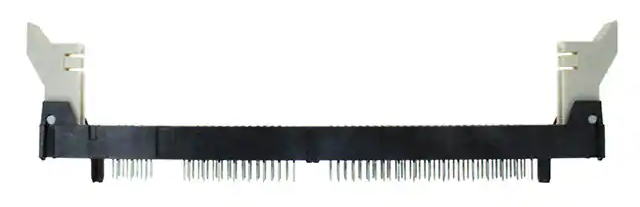
\includegraphics[scale=0.5]{Imagenes/DIMM100.png}
    \caption{Socket de conexión de cien pines de tipo DIMM-100, donde se inserta la controlCARD.}
    \label{dimm100}
\end{figure}

Estos pines de GPIO pueden ser configurados mediante un registro del DSC para cambiar su funcionalidad: cada pin cuenta con un multiplexor, de manera que, por ejemplo, el pin GPIO00 puede funcionar como pin de entrada/salida general, o bien como salida de la señal ePWM1A del módulo ePWM. Entonces, si observamos el \textit{pinout} de la controlCARD, podemos decidir cuáles pines del conector asignar para cada funcionalidad.\\

\paragraph{Salidas ePWM}

Como se mencionó en el capítulo \ref{analisis}, el TMS320F28335 cuenta con seis módulos ePWM, cada uno con dos salidas, A y B, es decir doce salidas totales. La controlCARD tiene pines asignados para cada una de estas salidas. En nuestro caso vamos a usar únicamente los primeros cuatro pines, correspondientes a las salidas ePWM1A, ePWM1B, ePWM2A y ePWM2B (Pines GPIO 0, 1, 2 y 3).\\

Estos pines se van a utilizar de manera que las dos salidas del módulo ePWM1 controlan la pata izquierda del puente, y las dos del módulo ePWM2 controlar la pata derecha. Las dos salidas de cada módulo se configuran para estar en contrafase, con un dead-time agregado entre estas señales de \SI[]{200}{\nano\second}. Luego, internamente se conecta la salida de sincronización SYNCO del primer módulo a la entrada de sincronización SYNCI del segundo módulo, y mediante el registro de fase del segundo módulo se controla su fase relativa a ePWM1, logrando una implementación del control de ciclo de trabajo mediante phase-shift que se explicó en la descripción del convertidor.\\

Las señales ePWM utilizadas, junto con las señales ePWM3A y ePWM3B (GPIO 4 y 5) del tercer módulo del DSC son conectadas también a una tira de pines para facilitar la medición de estas señales con un osciloscopio. Además, las señales del tercer módulo se pueden utilizar para implementar una funcionalidad adicional por fuera de los componentes de la placa.\\

\paragraph{Entradas de ADC}

Para la entrada de datos proveniente del sensor de efecto hall TMCS1100A4, se utiliza el módulo del conversor analógico digital de 12 bits y \SI[]{80}{\nano\second} de tiempo de conversión que se describió en el capítulo \ref{analisis}. Nuevamente, la controlCARD tiene pines asignados para cada una de las 16 (8 por cada canal A y B) entradas del conversor analógico-digital.\\

Para los datos del sensor se utiliza la primer entrada del canal A, ADCIN-A0, y se conectó una tira de pines a las tres primeras entradas del convertidor, hasta ADCIN-A2. Esto cumple el mismo propósito que la tira de pines para las señales ePWM.\\

\paragraph{Comunicación Serie}

Todos los controladores de la serie C2000 implementan cuatro protocolos de comunicación serie distintos: un bus {\Medium I\textsuperscript{2}C} (\textit{Inter-Integrated Circuit}), una interfaz {\Medium SPI} (\textit{Serial Peripheral Interface}), un módulo {\Medium SCI} (\textit{Serial Communications Interface}) más conocido como UART, y un módulo {\Medium McBSP} (\textit{Multichannel Buffered Serial Port}). El único protocolo que no se va a utilizar en esta plataforma es el de McBSP.\\

\subparagraph{I\textsuperscript{2}C}

El módulo I\textsuperscript{2}C, utilizado para transmitir los datos de tensión, corriente y potencia que entrega el LM5056A, se describió en detalle en el capítulo del sistema de medición. Las líneas de datos SDA y de reloj SCL estan multiplexadas a los pines GPIO 32 y 33 del controlador respectivamente. El cálculo de las resistencias de pull-up y el circuito de separación de la línea de datos ya se trató en el análisis detallado del protocolo.\\

Ambas líneas del bus también tienen salida a través de una tira de pines, para facilitar la evaluación del funcionamiento del bus, y conectar dispositivos adicionales, si se llegara a requerir.\\

\subparagraph{SCI (UART)}

El protocolo SCI, mejor conocido como UART (\textit{Universal Asynchronous Reciever-Transmitter}), es un bus de transmisión de datos en serie, asincrónico (sin señal de reloj para sincronizar), y full-duplex (capacidad de transmitir datos en ambas direcciones simultáneamente). Es un protocolo de velocidad de transmisión variable, y es común su utilización para la comunicación entre un controlador y dispositivos periféricos.\\

El TMS320F28335 cuenta con tres módulos independientes para comunicación por SCI (módulos A, B y C). En la plataforma se utilizó un único módulo para la transmisión de datos mediante el puerto USB. Esto se implementó mediante un integrado que convierte los datos que ingresan por el puerto a un formato para ser transmitido por UART. Las líneas de recepción SCIRX-A y transmisión SCITX-A del primer módulo corresponden a los puertos GPIO 28 y 29 respectivamente. Adicionalmente, al igual que el I\textsuperscript{2}C, se conectaron ambas líneas a una tira de pines.\\

\subparagraph{SPI}

La interfaz SPI es un protocolo de transmisión de datos en formato serie, sincrónico y full-duplex desarrollado por Motorola, y es generalmente utilizado para comunicaciones de corta distancia en sistemas embebidos. Es un bus multi-dispositivo y de esquema maestro/esclavo que cuenta con cuatro lineas: SPI-SIMO, para transmisión de datos del maestro hacia el esclavo; SPI-MISO, para transmisión de datos del esclavo hacia el maestro; SPI-CLK para transmitir la señal de reloj; y SPI-STE, que implementa un \textit{chip-select} para seleccionar el esclavo correcto.\\

En el controlador, este protocolo se implementa para conectar un módulo para lectura y escritura de tarjeta SD (se suelen vender módulos completos que incluyen la traducción de datos al formato SPI), con el propósito de almacenar datos en caso que fuera necesario. Las cuatro líneas del protocolo son implementadas en los puertos GPIO 16, 17, 18 y 19 respectivamente.\\

\subsubsection{Puerto JTAG}

\lipsum[1]\\

\subsubsection{Comunicación por USB}

\lipsum[2]\\

\begin{figure}[h]
    \centering
    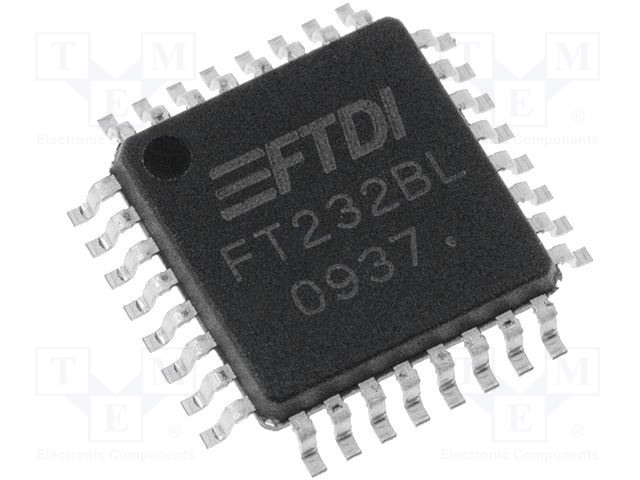
\includegraphics[scale=0.2]{Imagenes/FT232BL.jpg}
    \caption{Convertidor USB-UART para la implementación de una conexión USB, modelo FT232BL de FTDI Chip, en su encapsulado LQFP-32.}
    \label{ft232bl}
\end{figure}

\lipsum[3]\\

\subsubsection{Entrada/Salida General}

\lipsum[4]\\